%Computing counts, N1+ of several flavours of different sized n-grams.

The key requirements for computing probability under a Kneser-Ney language model are two types of counts: raw frequencies of \ngrams and occurrence counts, quantifying how many different contexts the \ngram has occurred in.
Figure~\ref{fig-counts-example} (right) illustrates the requisite
counts for calculating the probability of an example 4-gram.
In electing to store the corpus directly in a suffix tree, we need to provide mechanisms for computing these counts based on queries into the suffix tree.

\begin{figure*}[tpb]
\centering
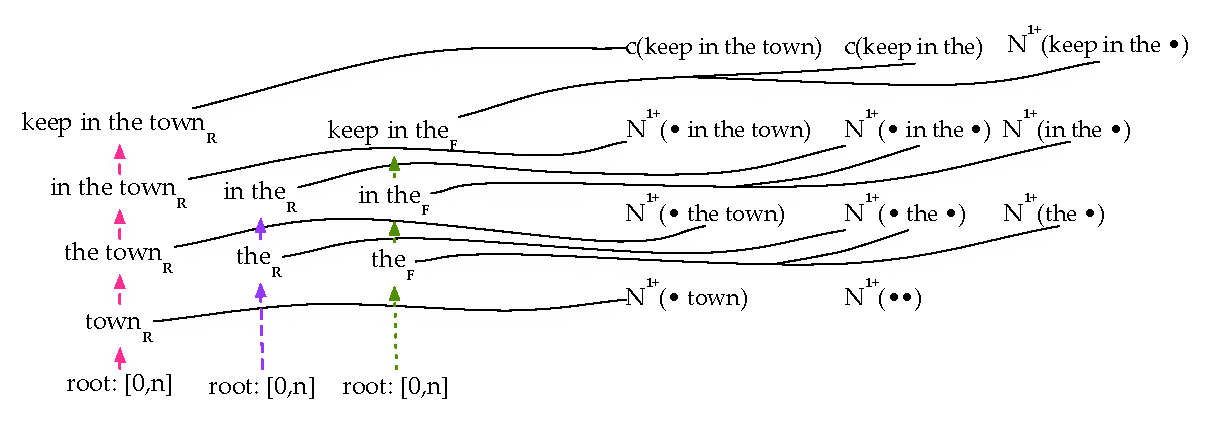
\includegraphics[width=0.85\textwidth]{figures/kn_dual_cst}
\vspace{-3ex}
\caption{Counts required for computing $P(\text{\em town} | \text{\em keep in the})$ (right) and the suffix tree nodes required for computing each value (left). The two left-most columns correspond to $\nrfull$ and $\nr$ and are updated using \emph{forward-search} in the reverse \CST, while the righter-most column correspond to $\nf$ and is updated using \emph{backward-search} in the forward \CST. See Algorithm~\ref{alg:pkn} for details.}
\label{fig-counts-example}
\end{figure*}


The raw frequency counts are the simplest to compute. First we
identify the locus node $v$ in the suffix tree for the query
\ngram; the frequency corresponds to the node's \emph{size}, an $\Order{1}$ 
operation which returns the number of descendents of $v$ \ehsan{Descendents or leaves of the subtree rooted at the node? This is not consistent with the size defined earlier on page 2.}. To illustrate, consider
searching for $c(\text{\emph{the night}})$ in  Figure~\ref{fig-suffix-tree}, which
matches a node with two descendents (labelled 19 and 12), and thus $c=2$. 

More problematic are the occurrence counts, which come in several
flavours: right contexts, $\nlplus{\patdot}$,
left contexts,  $\nlplus{\dotpat}$, and contexts to both sides of the pattern,
$\nlplus{\dotpatdot}$. 
The first of these can be handled easily, as 
\begin{equation*}
\nlplus{\patdot} = \left\{ 
\begin{array}{ll}
   \degree{t}{v}, \quad & \text{if~} \alpha = \pathlabel{t}{v} \\
   1, & \text{otherwise}
\end{array} \right.
\end{equation*}
where $v$ is the node matching $\alpha$, and 
$\pathlabel{t}{v}$ denotes the  {\it path-label} of $v$.%
\footnote{See the \supp for the explicit algorithm, but note there are some corner cases involving sentinels \#
  and \$, which must be excluded when computing occurrence counts.
  Such tests have been omitted from the presentation for clarity. On publication the
  source code will be released with the complete implementation (totalling 1k lines of C++).}
For example, \emph{keep in} has two child nodes in  Figure~\ref{fig-suffix-tree},
and thus there are two unique contexts in which it can occur, $\nlplus{\emph{keep in~}\Bigcdot}=2$,
while \emph{the keep} partially matches an edge in the forward suffix tree in
Figure~\ref{fig-suffix-tree} as it can only be followed by \emph{in}, $\nlplus{\emph{the keep~}\Bigcdot}=1$.
% This follows naturally from the suffix tree construction, where all descendent nodes correspond to larger \ngrams with same prefix, and each child edge extends the \ngram with a different subsequent symbol. 
% This method is illustrated in Algorithm~\ref{alg-nlplus}, which computes $\nlplus{\dotpat}$ 
% when $t$ is the reversed \CST and $\nlplus{\patdot}$ when $t$ is the forward \CST.
A similar line of reasoning applies to computing $\nlplus{\dotpat}$. 
Assuming we also have a second suffix tree representing the \emph{reversed corpus}, we first identify the reversed pattern (e.g., \emph{in keep}$_R$) and then use above method to compute the occurrence count (denoted hereafter $\nlplusfunc{t}{v}{\alpha}$, where $t$ is the \CST.). 

The final component of the Kneser-Ney LM computation is
$\nlplus{\dotpatdot}$, the number of unique contexts considering
symbols on both sides of the pattern. 
Unfortunately this does not map to a simple suffix tree operation,
but instead requires enumeration,
$\nlplus{\dotpatdot} = \sum_{s \in F(\alpha)} \nlplus{\dotpat s}$, 
where $F(\alpha)$ is the set of symbols that can follow $\alpha$.
%\end{equation*}
Algorithm~\ref{alg-occ-two-sided} shows how this is computed, with lines 7 and 8 enumerating $s \in F(\alpha)$ using the \emph{edge} labels of the children of $v$.
For each symbol, line 9 searches for an extended pattern incorporating
the new symbol $s$ in the reverse \CSA (part of the reverse \CST), by
refining the existing match $\nr$ using a single backward search
operation after which we can compute $\nlplus{\patdot
  s}$.\footnote{Backward search in the reverse tree corresponds to
  searching for the reversed pattern appended with one symbol.}
% Finally we can query the unique left contexts for the node (line 10),
% which we accumulate to yield the return value.
Line 5 deals with the special case where the pattern does not match a complete edge, in which case there is only only unique right context and therefore $\nlplus{\dotpatdot} = \nlplus{\dotpat}$.

\begin{algorithm}[t]
  \caption{Two-sided occ., $\nlplus{\dotpatdot}$ 
    \label{alg:n1plusfb}}
\footnotesize
  \begin{algorithmic}[1]
    \Require{$\nf$ in forward \CST $\tf$ matches $\alpha$}
    \Require{$\nf$ in reverse \CST $\tr$ matches $\alpha$}
    \Function{N1PlusFrontBack}{$\tf, \nf, \tr, \nr, \alpha$} 
        \Let{$o$}{$0$}
        %\If{$\leaf{\tf}{\nf} \, \vee \, \depth{\tf}{\nf} > |\alpha|$}   \Comment{leaves and patterns internal to an edge}
        \Let{$d$}{$\depth{\tf}{\nf}$}   
        \If{$d > |\alpha|$}   %\Comment{patterns internal to an edge}
          \Let{$o$}{$\nlplusfunc{\tr}{\nr}{\dotpat}$} %\Comment{have only one right context}
        \Else
           \For{$\chf \gets \children{\tf}{\nf}$} 
              \Let{$s$}{$\edge{\tf}{\chf}{d+1}$} %\Comment{find the first symbol on the edge label}
              \Let{$\chr$}{$\backwardsearchnode{\tr}{\nr}{s}$} %\Comment{find child node in reverse \CST}
%              \Statex    %\Comment{$\ar$ is the \CSA component of $\tr$}
              \Let{$o$}{$o + \nlplusfunc{\tr}{\chr}{\dotpat s}$}
            \EndFor
        \EndIf
      \State \Return{$o$}
    \EndFunction
  \end{algorithmic}
\label{alg-occ-two-sided}
\end{algorithm}

\nlplusname\ and \nlplusfrontbackname\ can compute the requisite occurence counts for \ngram language modelling, however at considerable cost in terms of space and time. 
The need for twin reverse and forward \CSTs incurs a significant storage overhead, as well as the search time to match the pattern in both \CSTs. 
We show in Section \ref{sec-single-cst}  how we can avoid the need for the reversed suffix  tree, giving rise to lower memory requirements and faster runtime. 
Beyond the need for twin suffix trees, the highest time complexity calls are \emph{string-depth}, \emph{edge} and \emph{backward-search}.
Calling \emph{string-depth} is constant time for internal nodes, but $\Order{\SASAMPLE \log\sigma}$ for leaf nodes; fortunately we can avoid this call for leaves, which by definition extend to the end of the corpus and consequently extend further than our pattern.\footnote{We assume search patterns do not extend beyond a single sentence, and thus will always be shorter than the edge labels.}
The costly calls to \emph{edge} and \emph{backward-search} however cannot be avoided.
This leads to an overall time complexity of $\Order{1}$ for \nlplusname\ and $\Order{F(\alpha) \times \SASAMPLE \times \log\sigma}$ for \nlplusfrontbackname, where $F(\alpha)$ is the number of following symbols and \SASAMPLE is the suffix array value sample rate described
in Section~\ref{sec-suffix}.

\section{Dual \CST Algorithm} 
\label{sec-dual-cst}

The methods above for computing the frequency and occurrence
counts provide the ingredients necessary for computing \ngram language model
probabilities. This leaves the algorithmic problem of efficiently ordering the search 
operations in forward and reverse \CST structures.

This paper considers an interpolated LM formulation, in which
probabilities from higher order contexts are interpolated with lower
order estimates.
% Our approach starts by querying the target word unigram $w_k$ and
% empty context $\emptyset$, from which the unigram probability can be computed
% Both patterns are extended to the left with symbol $w_{k-1}$, to form
% a bigram and the context unigram.
% In each step the probability is computed before extending the pattern,
% stopping after a fixed number of steps, $n$, or on encountering an
% unseen context.
This iterative process is apparent in Figure~\ref{fig-counts-example} (right) which shows the quantities required for probability scoring for an example \ngram.
Equivalently, the iteration can be considered in reverse, starting from unigram estimates and successively growing to large \ngrams, in each stage adding a single new symbol to left of the pattern. 
This suits incremental search in a \CST in which search bounds are
iteratively refined, which has a substantially lower time complexity
compared to searching over the full index in each step.
%This fits well with cheaply searching a \CST one symbol at a time.  


\begin{algorithm}[tpb]
  \caption{KN probability $P\big(w_k | w^{k-1}_{k-(m-1)}\big)$
    \label{alg:pkn}}
\footnotesize
  \begin{algorithmic}[1]
    \Function{ProbKneserNey}{$\tf, \tr, \ws, m$} 
        \Let{$\nf$}{$\rooot{\tf}$} \Comment{match for suffix of $w^{k-1}_{k-(m-1)}$}
        \Let{$\nr$}{$\rooot{\tr}$} \Comment{match for suffix of $w^{k-1}_{k-(m-1)}$}
        \Let{$\nrfull$}{$\rooot{\tr}$} \Comment{match for suffix of $w^{k}_{k-(m-1)}$}
        \Let{$p$}{$1$}
        \For{$i \gets 1 \text{ to } m$}
          \Let{$\nrfull$}{$\forwardsearchnode{\tr}{\nrfull}{w_{k-i+1}}$} %\Comment{update matches in \textsc{Cst}s}
          \If{$i > 1$}
             \Let{$\nf$}{$\backwardsearchnode{\tf}{\nf}{w_{k-i+1}}$} %\Comment{update context match in fwd \CST}
              \If{$i < m$}
             \Let{$\nr$}{$\forwardsearchnode{\tr}{\nr}{w_{k-i+1}}$} %\Comment{update context match in rev \CST}
          \EndIf
          \EndIf
          \Let{$D_i$}{lookup discount for $i$gram}
          \If{$i = m$} % or if s == '<s>' 
%                 \Comment{compute frequency count and denominator}
             \Let{$c$}{$\size{\tr}{\nrfull}$} 
             \Let{$d$}{$\size{\tf}{\nf}$}
          \Else  %\Comment{compute occurrence count and denominator}
             \Let{$c$}{$\nlplusfunc{\tr}{\nrfull}{\Bigcdot w^{k}_{k-i+1}}$} 
             \Let{$d$}{}
             \Statex \hfill $\nlplusfrontbackfunc{\tf}{\nf}{\nr}{\Bigcdot w^{k-1}_{k-i+1} \Bigcdot}$ %\Comment{precompute $\nlplus{\Bigcdot\Bigcdot}$}
           \EndIf
           \If{$i > 1$}
             \If{$\nf$ is valid} %\Comment{compute backoff probability, or backoff for unseen contexts}
                  \Let{$q$}{$\nlplusfunc{\tf}{\nf}{w^{k-1}_{k-i+1} \Bigcdot}$}  %\Comment{defined as $0$ for $i=1$}
                  \Let{$p$}{ $\frac{1}{d} \left( \max(c-D_i, 0)  + D_i  q  p \right)$} 
               \EndIf
          \ElsIf{$i = 1$}
              \Let{$p$}{$c  / \nlplus{\Bigcdot\Bigcdot}$}
          \EndIf
        \EndFor
      \State \Return{$p$}
    \EndFunction
  \end{algorithmic}
\label{alg-kn-slow}
\end{algorithm}



%\afterpage{\clearpage}

Algorithm~\ref{alg-kn-slow} presents an outline of the approach.
This uses a forward \CST, $\tf$, and a reverse \CST, $\tr$, with three \CST nodes (lines 2--4) tracking the match progress for the full $i$gram ($\nrfull$) and the $(i-1)$gram context ($\nf, \nr$), $i=1 \ldots m$.
The need to maintain three concurrent searches arises from the calls to \emph{size}, $\nlplus{\dotpat}$, $\nlplus{\patdot}$ and $\nlplus{\dotpatdot}$ (lines 14, 15; 17; 21; and 18, respectively).
These calls impose conditions on the direction of the suffix tree, e.g., such that the edge 
labels and node degree can be used to compute the number of left or right contexts in which a pattern appears. 
The matching process is illustrated in Figure~\ref{fig-counts-example} where the three search nodes are shown on the left, considered bottom to top, and their corresponding count operations are shown to the right.
The $\nlplus{\dotpat}$ calls require a match in the reverse \CST (left-most column, $\nrfull$), while the $\nlplus{\patdot}$ require a match in the forward \CST (right-most column, $\nf$, matching the $(i-1)$gram context). 
The $\nlplus{\dotpatdot}$ computation reuses the forward match while also requiring a match for the $(i-1)$gram context in the reversed \CST, as tracked by the middle column ($\nr$).
Because of the mix of forward and reverse \CSTs, coupled with search patterns that are revealed right-to-left, incremental search in each of the \CSTs needs to be handled differently (lines 7--11).
In the forward \CST, we perform \emph{backward search} to extend the search pattern to the left, which can be computed very efficiently from the BWT in the \CSA.\footnote{See \supp Table~1 for the time complexities of this and other \CSA and \CST methods.}
Conversely in the reverse \CST, we must use \emph{forward search} as we are effectively extending the reversed pattern to the right; this operation is considerably more costly.

The discounts $D$ on line 12 of Algorithm~\ref{alg-kn-slow} and
$\nlplus{\Bigcdot\Bigcdot}$ (a special case of line 18) are precomputed directly from the \CSTs thus avoiding several costly computations at runtime. 
The precomputation algorithm is provided in Algorithm~8 in the \supp,
and operates by traversing the nodes of the reverse \CST and at each
stage computing the number of \ngrams that occur 1--4 times or with
$\nlplus{\dotpat} \in [1,4]$, for various lengths of \ngrams.
These quantities are used to compute the discount parameters, which
are then stored for later use in inference.\footnote{Discounts are computed up to a limit on \ngram size, here set to 10. The highest order values are used for computing the discount of \ngrams above the limit at runtime.}
Note that the \textsc{PrecomputeDiscounts} algorithm can be slow,
although it is significantly faster if we remove the \emph{edge} calls
and simply include in our counts all \ngrams finishing a sentence or
spanning more than one sentence.
This has a neglibile (often beneficial) effect on perplexity.
%These approximate discounts are typically within $10^{-2}$ of the correct values.

\section{Improved Single \CST Approach}
\label{sec-single-cst}

The above dual \CST algorithm provides an elegant means of computing LM probabilities of arbitrary order and with a limited space complexity ($\Order{n}$, or roughly $n$ in practice).
However the time complexity is problematic, stemming from the expensive method for computing \nlplusfrontbackname and repeated searches over the \CST, particularly \emph{forward-search}.
Now we outline a method for speeding up the algorithm by doing away with the reverse \CST.
Instead the critical counts, $\nlplus{\dotpat}$ and $\nlplus{\dotpatdot}$ are computed directly from a single forward \CST. 
This confers the benefit of using only backward search and avoiding redundant searches for the same pattern (cf.~lines 9 and 11 in Alg~\ref{alg-kn-slow}).


The full algorithm for computing LM probabilities is given in the \supp as Algorithm 7, however for space reasons we will not describe this in detail.
Instead we will focus on the method's most critical component, the algorithm for computing $\nlplus{\dotpatdot}$ from the forward \CST, presented in Alg~\ref{alg:n1plusfb_wt}.
The key difference from Alg~\ref{alg:n1plusfb} is the loop from lines 6--9, which uses the \emph{interval-symbols} method.
This method assumes a \emph{wavelet tree} representation of the \SA component of the \CST, an efficient encoding of the BWT as describes
in section~\ref{sec-css}.
%\emph{Burrows-Wheeler transform} (an array comprising the symbol preceeding each entry in the \SA).
The \emph{interval-symbols} method uses \rankop~and \selectop~bit operations to efficiently identify for a given pattern the set of preceeding symbols, and for each of symbol its range of occurrences in the \SA.
Using the same process as backward search, described in Section~\ref{sec-cst}, these ranges can be used to find the $\SA[l,r]$ interval for the extended pattern (lines 7 and 8), which uniquely deterimines the corresponding suffix tree node.
To illustrate, consider the pattern $\alpha=\text{``night''}$ in Figure~\ref{fig-suffix-tree}.
From the BWT we can see that this is preceeded by $s=$``old'' (1$^{st}$ occurrence in the BWT) and $s=$``the'' (4$^{th}$ and $5^{th}$);
from which we can compute the suffix tree nodes, namely
$[15,15]$ and $[16+(4-1),16+(5-1)] = [19,20]$ for ``old'' and ``the'' respectively.\footnote{Using the offsets into the \SA for each symbol, $C_{\text{old}} = 15$ and $C_{\text{the}} = 16$, while $-1$ adjusts for counting from 1.}
%$C_{\text{the}} = 16$ (``the'' corresponds to \SA entries 16--20) and therefore the location of ``the night'' is $[16+(4-1),16+(5-1)] = [19,20]$.\footnote{Subtracting one to adjusts for counting from 1 in the above exposition, not 0.}
%For example, in Figure~\ref{fig-suffix-tree} the pattern $\alpha=\text{``night''}$ is preceeded by $s=$``old'' and $s=$``the''.
%These correspond to the only occurrence of ``old'', and the 4$^{th}$ and 5$^{th}$ occurrence of ``the'' in the BWT.
%These occurence bounds can then be used to calculate the range in the \SA by adding to $C_s$, the precomputed offset of the first pattern beginning with $s$, exploiting the property that the \SA is lexicographically sorted.
%In the example above, $C_{\text{the}} = 16$ (``the'' corresponds to \SA entries 16--20) and therefore the location of ``the night'' is $[16+(4-1),16+(5-1)] = [19,20]$.\footnote{Subtracting one to adjusts for counting from 1 in the above exposition, not 0.}


\begin{algorithm}[t]
  \caption{%Two-sided occ, 
$\nlplus{\dotpatdot}$, using forward \CST 
    \label{alg:n1plusfb_wt}}
\footnotesize
  \begin{algorithmic}[1]
    \Require{$\nf$ in forward \CST $\tf$ matches $\alpha$}
%    \Require{the \CSA component, $\af$ of $\tf$ is a wavelet tree}
    \Function{\nlplusfrontbacklname}{$\tf, \nf, \alpha$} 
        \Let{$o$}{$0$}
        %\If{$\leaf{\tf}{\nf} \, \vee \, \depth{\tf}{\nf} > |\alpha|$}   
        \If{$\depth{\tf}{\nf} > |\alpha|$}   
          \Let{$o$}{$\nlplusbacklfunc{\tf}{\nf}{\dotpat}$} %\Comment{only one unique right context}
        \Else
            \For{$\langle l, r, s\rangle \gets \intervalsymbols{\tf}{\lb{\nf}}{\rb{\nf}}$}
               \Let{$l'$}{$C_s + l$}% \Comment{compute offsets into \SA for patterns starting with symbol $s$}
               \Let{$r'$}{$C_s + r$} %\Comment{adjusted by occurence indices $[l,r]$}
               \Let{$o$}{$o + \nlplusbacklfunc{\tf}{\text{node}(l', r')}{\dotpat s}$}
            \EndFor
          \EndIf
      \State \Return{$o$}
    \EndFunction
  \end{algorithmic}
\end{algorithm}

\nlplusbacklname is computed in a similar way, using the \emph{interval-symbols} method to compute the number of unique preceeding symbols (see \supp, Algorithm~6).
Overall the time complexity of inference for both \nlplusbacklname and \nlplusfrontbacklname is $\Order{k \log \sigma}$ where $k$ is the number of preceeding symbols, a considerable improvement over \nlplusfrontbackname using the forward and reverse \CSTs.
Overall this leads to considerably faster computation of \ngram probabilities compared to the two \CST approach, and although still slower than highly optimised LM toolkits like \textsc{Srilm}, it is fast enough to support large scale experiments, and has considerably better scaling performance with the Markov order $m$ (even allowing unlimited order), as we will now demonstrate.


%%% Local Variables: 
%%% mode: latex
%%% TeX-master: "cstlm"
%%% End: 
